\documentclass[11pt]{article}
\usepackage{icmlko}
\begin{document}

\title{만화 바닥 아래에서도 축이 통한다 --- 고친 규칙의 네 번째 점}
\author{월드모델 실험실}
\date{노트 386 · 2026년 8월 1일}
\maketitle

\begin{abstract}
노트 385가 규칙을 고쳤다 --- \emph{위를 뜬 것 자체는 도메인 점수를 안
부풀린다. 부풀리는 것은 잘려 나간 구간에서 축이 안 통할 때다.} 그때
점이 셋이었다(게임 $+0.2746$ 통함 · 세계애니 $+0.0223$ 안 통함 · 펀딩
$-0.0094$ 안 통함). 네 번째를 쟀다.

만화는 무게 258 · 바닥 633(서재 등록 수)이고 한 번도 아래를 안 봤다.
AniList 의 \texttt{popularity\_lesser: 633} $+$
\texttt{startDate\_greater: 20241231} 로 2025년 이후 바닥 아래 999편을
받아, 국가 필터를 통과한 421편을 \emph{유보에만} 넣고 학습 1,783행은
고정했다.

\begin{center}
\begin{tabular}{lrrr}
\hline
무리 & 행 & 라벨 퍼짐 & $\rho$ \\
\hline
바닥 위 (옛) & 258 & 0.264 & $+0.2503$ \\
\textbf{바닥 아래} (새) & 421 & 0.143 & $\mathbf{+0.1046}$ \\
\hline
\end{tabular}
\end{center}

아래쪽 퍼짐이 위의 절반이라 노트 376의 연속 창 대조를 돌렸다: 위쪽에서
같은 퍼짐(0.143$\pm$0.04)의 라벨 순 연속 창 7,800개의 중앙이 $+0.0921$,
5\,--\,95\%가 $[+0.0114,\ +0.1965]$ 다. \textbf{바닥 아래는 59번째 백분위
--- 띠 한가운데다.} 같은 퍼짐에서 위와 아래가 똑같이 통한다.

\textbf{그러므로 만화 점수는 안 부풀었다.} 고친 규칙의 네 점이 둘씩
갈린다 --- 게임 · 만화는 통하고(점수 정상), 세계애니 · 펀딩은 안 통한다
(펀딩은 실제로 4.8배 부풀어 있었고 세계애니는 넓힐 수 없었다).

\textbf{넓히지는 않는다.} 새 421행에 신호가 있으니 노트 376이 세계애니를
거절한 이유는 여기 없다. 그런데 합쳐서 재면 $+0.0892$ 로 \emph{양쪽 어느
것보다도 낮다} --- 두 무리 라벨 중앙이 1,133 대 324 라 수준 차가 순위를
흔든다. 노트 384가 게임에서 본 것과 \emph{반대 부호의} 같은 함정이다.
\textbf{합친 수가 못 믿을 수라 그 수로 분모를 바꾸지 않는다.}
\end{abstract}

\section{어떻게 받았나 --- 두 번 막혔다}

\textbf{첫 시도는 못 닿았다.} 노트 376이 세계애니에 쓴 방법(인기 내림차순
쪽 61\,--\,160)을 그대로 돌렸더니 2,000편이 왔는데 popularity 최소가
\textbf{2,648} 이었다 --- 우리 바닥 633 보다 한참 위다. AniList 쪽매김이
5,000건에서 끊긴다.

\textbf{그래서 우리 표본이 어떻게 633까지 내려가 있는지부터 물었다.}
가설은 라벨 표류였다 --- 서재 등록 수는 쌓이는 값이니 수집 당시 값이
낮았을 수 있다. \textbf{틀렸다.} 우리 2,983편 중 현재 목록에 있는
2,478편의 저장값 대 현재값이 중앙 \textbf{1.00배} · 순위 상관
$\mathbf{+1.0000}$ 이다. 값은 안 변했다.

진짜 이유는 \textbf{새 작품이 들어와 경계가 올라간 것}이다. 우리 505편은
수집 당시 상위 5,000 안이었는데 지금은 밖이다. 값이 그대로여도 순위는
내려간다. \textbf{누적 라벨이 위험한 방식이 하나 더 있다} --- 노트 209가
``오래된 것일수록 크다''를 잡았다면 이것은 ``같은 값도 시간이 지나면
순위가 내려간다''다.

\textbf{두 번째 시도가 통했다.} 쪽매김 대신 값으로 거른다 ---
\texttt{popularity\_lesser: 633} 이면 5,000 한계와 무관하게 바닥 아래로
곧장 간다. 받은 999편의 popularity 가 201\,--\,632, 2025년 793편 ·
2026년 207편이다.

\begin{figure}[t]
\centering
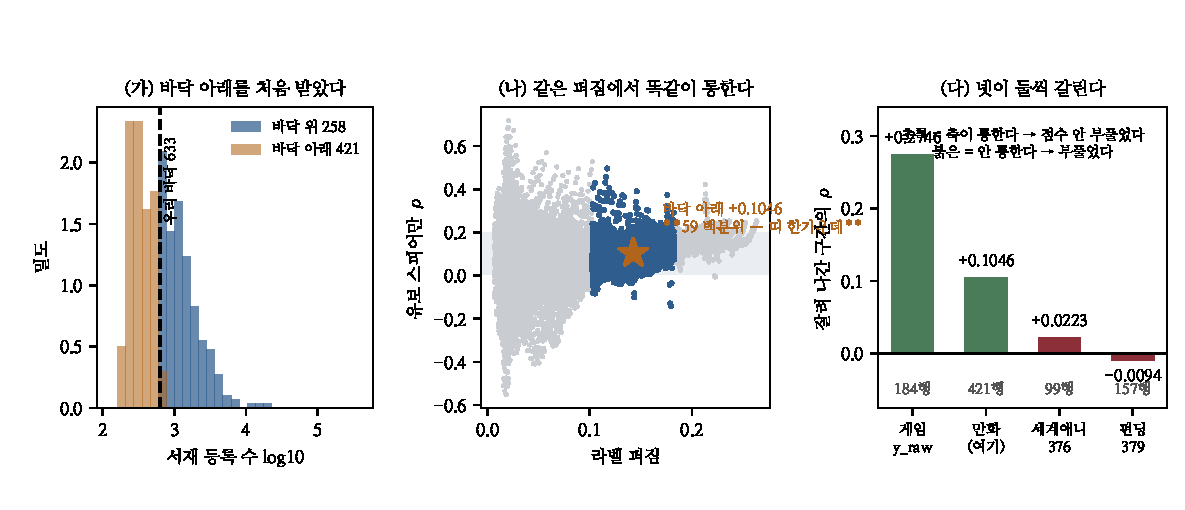
\includegraphics[width=\linewidth]{figs/fig386.pdf}
\caption{\textbf{(가)} 바닥 위 258행과 처음 받은 바닥 아래 421행의 라벨
분포. \textbf{(나)} 위쪽에서 같은 퍼짐의 연속 창 7,800개(파랑)와 그
5\,--\,95\% 띠. 바닥 아래(별)는 59번째 백분위다. \textbf{(다)} 고친 규칙의
네 점 --- 잘려 나간 구간에서 축이 통하는 둘과 안 통하는 둘.}
\label{fig:main}
\end{figure}

\section{쟀다}

절차는 노트 372 · 376 · 379와 같다 --- 새 행은 유보에만, 학습은 고정,
\emph{한 번의 적합 안에서} 가른다. 축은 \texttt{ingest/manga\_axes.py} 를
그대로 돌려 만들었다. 저자 잡힌 비율이 새 행 100\% · 기존 100\% 라 배치
표시자가 안 생긴다(노트 354 · 379의 자리를 확인했다).

\textbf{위험 점검.} 옛 행의 공유 축 다섯이 99\,--\,100\% 그대로이고 라벨이
바뀐 행은 0이며, 새 421행 중 학습으로 가는 행이 0이다.

\textbf{퍼짐 대조.} 아래쪽 퍼짐이 0.143 으로 위(0.264)의 54\%라 노트 376의
실패 모드가 그대로 있다. 위쪽 258행을 라벨 순으로 정렬해 크기
$20\ldots258$ 의 연속 창을 전부 잘라(7,800개 중 퍼짐이 맞는 것) 띠를
만들었다. \textbf{바닥 아래 $+0.1046$ 은 그 띠의 59번째 백분위다} ---
중앙 $+0.0921$ 보다 오히려 살짝 높다.

\section{네 점이 둘씩 갈린다}

\begin{center}
\begin{tabular}{lrrl}
\hline
도메인 & 바닥 아래 행 & 그 구간 $\rho$ & 위쪽 점수가 부풀었나 \\
\hline
게임 (\texttt{y\_raw}, 노트 385) & 184 & $+0.2746$ & 아니다 ($p=0.794$) \\
\textbf{만화} (여기) & 421 & $\mathbf{+0.1046}$ (59\%ile) & \textbf{아니다} \\
세계애니 (노트 376) & 99 & $+0.0223$ & 넓힐 수 없었다 \\
펀딩 (노트 379) & 157 & $-0.0094$ & 그렇다 (4.8배) \\
\hline
\end{tabular}
\end{center}

\textbf{바닥의 높이는 여전히 답이 아니다.} 만화 바닥 633은 세계애니
19,533보다 훨씬 낮은데 만화는 멀쩡하고 세계애니는 안 된다. 게임 바닥
82는 제일 낮은데도 \texttt{y\_raw} 로 보면 82\%가 잘려 있었고 그래도
멀쩡하다. \textbf{재 봐야 안다는 것이 이 규칙의 전부이고, 그것이 값이다}
--- 노트 382가 만든 바닥 표로 우선순위를 정하려던 것은 헛수고였다.

\section{안 넓히는 이유}

새 421행에 신호가 있으니 노트 376이 세계애니를 거절한 근거(신호 0)는
여기 없다. 그래도 안 넓힌다.

\begin{center}
\begin{tabular}{lrr}
\hline
채점 & 행 & $\rho$ \\
\hline
바닥 위만 & 258 & $+0.2503$ \\
바닥 아래만 & 421 & $+0.1046$ \\
\textbf{합쳐서} & 679 & $\mathbf{+0.0892}$ \\
\hline
\end{tabular}
\end{center}

\textbf{합친 수가 양쪽 어느 것보다 낮다.} 두 무리 라벨 중앙이 1,133 대
324 라 수준 차가 순위를 흔든다 --- 노트 384가 게임에서 본 것(합치면
$+0.7450$ 으로 \emph{오른다})과 같은 함정의 반대 부호다. \textbf{합침이
어느 쪽으로 움직이든 그 수는 두 무리의 수준 차를 나른다.}

분모를 바꾸는 것은 자료 결정이고(노트 82 · 90) 재현도 되지만, \emph{무엇을
분모에 넣을지}는 ``2025년 이후 만화의 참 분포''를 알아야 정해진다. 우리가
가진 것은 위 258과 아래 421인데 실제 비율은 그것이 아니다. \textbf{비율을
모르면서 합치면 그 비율이 점수가 된다.} 지금 답할 수 없어 안 한다.

\section{남은 것}

\begin{center}
\begin{tabular}{lll}
\hline
항목 & 왜 값이 큰가 & 어떻게 \\
\hline
2025$+$ 만화 참 분포 & 그걸 알아야 분모를 정한다 & \texttt{popularity\_lesser} 로 구간별 총수 \\
아이돌 바닥 아래 & 남은 절단 도메인 & 무게 51 이라 값은 작다 \\
왜 어디선 통하나 & 규칙의 다음 층 & 네 도메인 축 덮음 · 라벨 성질 견주기 \\
순위 표류 & 같은 값도 순위가 내려간다 & 만화 505편이 그 예다 \\
\hline
\end{tabular}
\end{center}

\end{document}
